%MRC5December2012 -- Added a bit about  the corporate partner context
%Context
\chapter{Context}
\label{sec-context} %Label for cross-referencing

\section{Need Statement}
Airlines are always searching for new ways to fit more people on a single flight and increase their profit margin, making the seats in the aircraft smaller and closer. As the seats get smaller, the personal space for a passenger shrinks, making it harder for anyone to move and fit comfortably as shown in Figure \ref{fig:9}.

\begin{figure}[h]
  \centering
     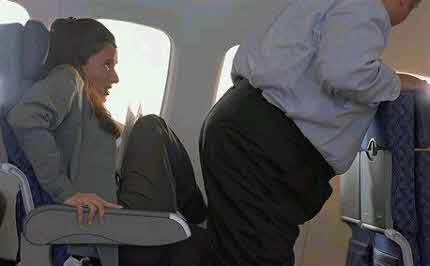
\includegraphics[width=7cm]{images/image009.png}
   \caption{With Airlines adding more and more seats to their planes, it is increasingly hard to maneuver around the cabin. \cite{2014airlines}}
  \label{fig:9}
\end{figure}


As global business continues to increase, people are constantly on the go and airports are becoming larger and larger, growing busier each year.  The distance from check-in to gate is increasing as more airlines expand terminals. Therefore, it becomes a problem for passengers who have a hard time walking long distances or need assistance with bags or a mobility device. More airport staff are needed to move the passengers with mobility needs, yet often the staff are not trained in handling the mobility devices or the person with disabilities.  

Additionally, airlines have  limited space in the cabin because of the increased amount of seats, requiring assistive devices to be stored in the cargo hold where they are susceptible to damage.  The flying experience today is tailored to a person that has all of his/her mobility, leaving out those who have some impairment that requires additional time. However, 58 million Americans live with a disability, including 5.5 million military veterans, so this is a problem we cannot ignore. %\cite{}

%Would it not be great if the flying experience were individually tailored to a person’s needs? What if the cabin could be %redesigned to improve the flying experience for the passengers with limited mobility as well as for the average passenger? %Such design would create an experience that is comfortable, making the airline and aircraft manufacturer more popular %among its customers because the final user, the passenger, is the one the plane is designed for.

\section{Problem Statement}
The biggest painpoints our users are facing (which are deeply analyzed in appendix A) can be broken down into the following two areas that need to be addressed:

\begin{list}{-}{}
  \item Mobility inside the Cabin
  \item Storage and Security of Assistive Devices
\end{list}

The whole process (see Appendix B) was analyzed and  we found that the current systems in place today are those required by the FAA and ADA regulations.  However, these systems have gaps that need to be addressed in order to improve the passenger experience.  The interviews we conducted during Autumn quarter showed the gaps and led to uncovering these two main pain points. Our users want to be able to transfer from their wheelchair to the aisle chair independently and without the interference of others and they especially don't want to be carried over a stranger's shoulder.  They also want to know that their wheelchair will be handled with the utmost care and returned to them in working condition with no damage at all.   

This is what our user needs and wants addressed in order to have a better flying experience that is more personal, allows for independence and control, and provides them with peace of mind. In addition, the airport staff and flight attendants need to be considered to ensure that they can use the new systems with ease and without an increased time committment by making the solution as intuitive and inclusive into the airport personnel's current tasks as possible. 


\section{Vision Statement}

Imagine you are packing for a trip and you pack your most important possession in your carry-on.   But when you arrive at the gate, you are required to gate check your bag.  You immediately panic. You do not know if the bag will be damaged. What if it gets lost? Put on the wrong flight? Your entire flight is ruined because now all you can think about is what state your bag will be when you arrive, especially since airlines do not have the best reputation concerning luggage handling. 

Now imagine if this was your wheelchair.  Your legs. Your independence. What if you had no clue how you were going to move now that you no longer have a functional wheelchair? What if your activity in the cabin was limited due to the loss of your chair?  For our users, this is a struggle every time they board a plane and have to endure a flight of misery and constant worry.  What if we could eliminate this unease, worry and fear by designing a new system that allows the user to know how their wheelchair was handled, to know it was safe, and that it will be there safely when they disembark?  What if we could design a way for them to be able to move in the cabin with ease and make the bathroom and other tasks more accessible? 

The two systems described in the story above are our vision and focus for the final product. Our users are in need of independence.  The current systems that are utilized today on airplanes and in airports require our users to be assisted by airport or airline personnel for any task that requires mobility.The user interviews from fall quarter stressed the importance of independence and the pain points that the lack of independence create in the flying experience.  Therefore, the theme of independence was the driving force behind the solution and design space described above. 

 With independence in mind, we found that mobility inside the cabin and the storage and security of the wheelchair were the two places where independence broke down the most in the flight experience. The pain point of mobility in the cabin is being addressed by redesigning the aisle chair.  The new aisle wheelchair will allow for user control during boarding and disembarking, for ease of independent transfer using a sliding seat, and for ease of mobility in the cabin such as using the restroom. The storage and security of the wheelchair will be accomplished with a specialized shipping container that allows for the wheelchair to be strapped or tied down in the jetway in front of the user. The user will be able to supervise the entire process and will receive updates of who is responsible for their chair as the container is loaded into the cargo hold.  These two solutions will be bringing independence and control back to our users and creating a more desirable experience. 

\section{Corporate Partner: Embraer}

\begin{figure}[h]
  \centering
     
\includegraphics[width=8cm]{images/image010.jpg}
  \label{fig:10}
\end{figure}

The corporate partner for this design project is Embraer.  Since 1969, Embraer has been involved in all aspects of the aviation field.  Embraer began with support from the Brazilian government to produce military aircraft in addition to its small passenger planes.  Embraer then expanded to agricultural planes and later to commercial planes and business/private jets.  Embraer has over 5,000 aircraft operating in over 80 countries.  They are the market leader for commercial jets with fewer than 120 seats.  Embraer is interested in expanding its commercial market to larger commercial jets, in maintaining some of the best executive jets, and in entering new defense markets.

\section*{Corporate Liaison}
Luciana Ribeiro Monteiro \\
  Technology Development \\
  Embraer - SJK \\
  Phone: +55 12 3927 8576 \\
  luciana.monteiro@embraer.com.br

\section{The Design Team}
Our team has a diverse educational, cultural, and social background that encompasses many skill sets and multiple areas of study. 

\subsection*{Stanford University}


\noindent 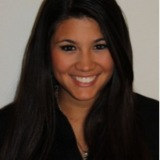
\includegraphics[width=40mm]{images/image011.jpg}
\parbox[b]{0.6\textwidth}{\textbf{Maria Barrera}\\
Status: Mechanical Engineering Graduate Student\\
Contact: mariabarrera5491@gmail.com\\
}

I was born in Colombia and moved to South Florida with my mom when I was 10. My dad and sister still live in Colombia so I tend to hop back and forth every chance I get. I did my undergraduate at Stanford also in Mechanical Engineering and have developed a deep interest for entrepreneurship during my time here. I run a tutoring company in the area and hope to one day start a company in the aviation sector. I also enjoy traveling, photography and playing with puppies!
\\ 


\noindent 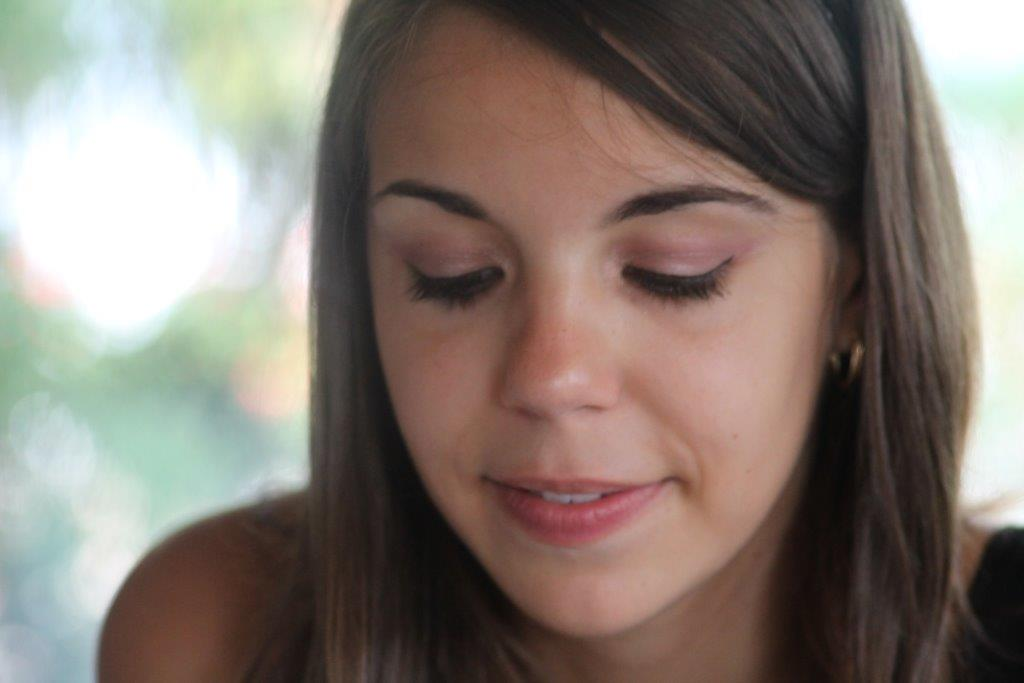
\includegraphics[width=40mm]{images/image012bis}
\parbox[b]{0.6\textwidth}{\textbf{Laura Hoinville}\\
Status: Aeronautics and Astronautics Graduate Student\\
Contact:  laurah31@stanford.edu \\
}

I come from Toulouse, France. I attended ISAE-Supaero (the French Graduate school of Aerospace Engineering) at Toulouse for my undergraduate degree in Aeronautics. I worked at Airbus head quarters in Blagnac, France as an intern last summer and want to make a career in the field of aircraft design. I'm also interested in dance (ballet, modern jazz, contemporary), gymnastics, scuba diving and reading.
\\ 


\noindent 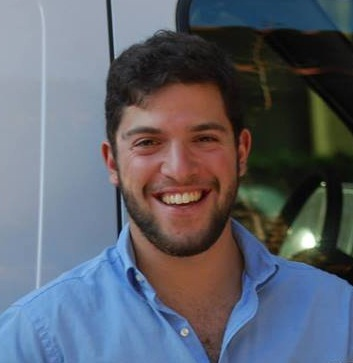
\includegraphics[width=40mm]{images/cliff.jpg}
\parbox[b]{0.6\textwidth}{\textbf{Cliff Bargar}\\
Status: Mechanical Engineering Graduate Student\\
Contact: cbargar@stanford.edu \\
Website: http://cliffbargar.com \\
}

Having spent the first 22 years of my life within a subway ride of Boston, Massachusetts, I decided to drive west and come to Stanford. I'm completing my MSME this spring, focusing on mechatronics, robotics, and controls. I graduated with a BSME from Tufts University, where I double majored in Mechanical Engineering and Mathematics, was an active member of Engineers Without Borders and the Tufts Robotics Club, and ran on the Tufts Cross Country and Track and Field teams. Here at Stanford I'm a Course Assistant for ME218 and a researcher in the CHARM lab as well as an active member of the Stanford Running Club.

\subsection*{University of S\~{a}o Paulo}

\noindent 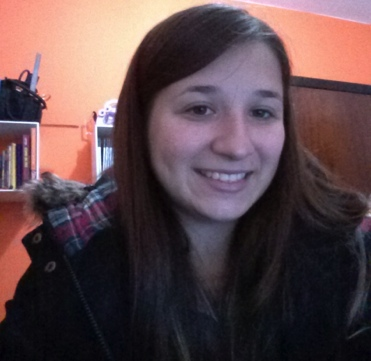
\includegraphics[width=40mm]{images/image013}
\parbox[b]{0.6\textwidth}{\textbf{Amanda Mota Almeida}\\
Status: Product Design Undergraduate Student\\
Contact: amandamotaalmeida@gmail.com \\
}

I was born and raised in S\~{a}o Paulo. I'm attending the University of S\~{a}o Paulo for my undergraduate studies in Product and Graphic Design. I have worked in a project with Embraer in the past regarding the design and comfort in the aircraft cabin (2011), I have interned for Staples in S\~{a}o Paulo – SP (2012) and I was part of exchange in Portugal last year (2013). My interests include: photography, arts and crafts and reading.
\\ 



\noindent 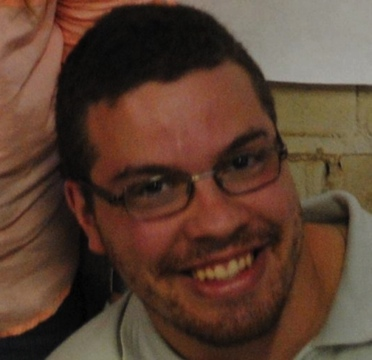
\includegraphics[width=40mm]{images/image015}
\parbox[b]{0.6\textwidth}{\textbf{Luiz Durao}\\
Status: Industrial Engineering Undergraduate Student \\
Contact: luiz.durao@usp.br  \\
}

I was born and raised in S\~{a}o Paulo city. I attended Colégio Etapa for my High School and it was while participating in the Chemistry and Physics Olympiads that I discovered my taste for the sciences. I'm attending the University of S\~{a}o Paulo for my undergraduate studies in Industrial Engineering. I have interned for GE Oil and Gas at Jandira – SP and I have worked since my sophomore year as a teaching assistant for some courses at USP. My interests include soccer, music and movies.
\\ 

\noindent 
\includegraphics[width=40mm]{images/image016}
\parbox[b]{0.6\textwidth}{\textbf{Guilherme Kok}\\
Status: Industrial Engineering Undergraduate Student \\
Contact:guilhermekok@gmail.com  \\
}

As a Brazilian and a soccer enthusiast, I grew up in S\~{a}o Paulo and in Baltimore. I've also spent 5 months in Nanaimo (Canada, BC) and 1 year studying at the University of Illinois at Urbana Champaign. I'm currently finishing my undergraduate studies at the University of S\~{a}o Paulo in Brazil, where I study Industrial Engineering. I have interned for a taxi app startup and have done undergrad research concerning the consolidation of the phonographic industry. My interests include playing soccer, hiking, tasting different cuisines and travelling, preferably to remote locations. 
\\

\noindent 
\includegraphics[width=40mm]{images/image014}
\parbox[b]{0.6\textwidth}{\textbf{Rodrigo Monteiro de Aquino}\\
Status: Computer Engineering Undergraduate Student \\
Contact: guigonyts@usp.br \\
}

I have lived all my life in S\~{a}o Paulo. I am now graduating in Computer Engineering at USP and I also work in a technology development lab at the university. I have worked on several projects developing educational games and other educational interfaces that help children learn with technological devices.  I like to play videogames and go to the movie theater. I like science fiction movies and reading adventure books.
\\ 


\section{Contributors}

\noindent 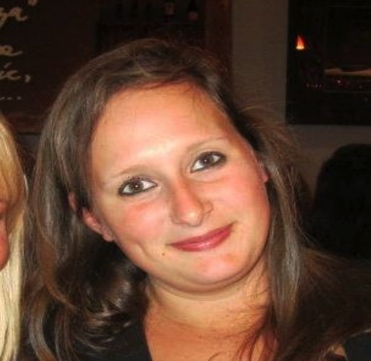
\includegraphics[width=40mm]{images/image012.jpg}
\parbox[b]{0.6\textwidth}{\textbf{Erika Finley}\\ \\
Contact: erikam.finley@gmail.com  \\
}

I was born and raised in Tennessee. I attended the University of Tennessee at Knoxville for my undergraduate degree in Mechanical Engineering. I participated in a study abroad in Canberra, Australia. I have interned for Tennessee Valley Authority at Browns Ferry Nuclear Plant and for Schlumberger at the Rosharon Design Center. I will be interning at Microsoft this upcoming summer. My interests include baking, reading, photography, and roller coasters.
\\

\noindent 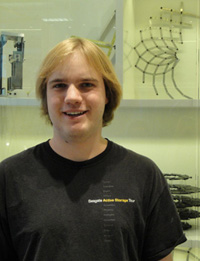
\includegraphics[width=40mm]{images/robert_karol.jpg}
\parbox[b]{0.6\textwidth}{\textbf{Robert Karol}\\ \\
Contact: robbiekarol@gmail.com  \\
}

I grew up in New Jersey through high school. After that, I moved to southern california where I attended the California Institute of Technology majoring in Mechanical Engineering with minors in Aerospace Engineering and Control and Dynamical Systems. I have worked on robotics projects with NASA’s Jet Propulsion Laboratory, as well as experiments in high altitude photography and performed research in microgravity.
\\

\noindent 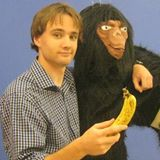
\includegraphics[width=40mm]{images/riley.jpg}
\parbox[b]{0.6\textwidth}{\textbf{Riley Shear}\\ \\
Contact: rjshear@gmail.com
}

Riley is finishing an MS in ME at Stanford University, where he came for graduate study after obtaining a BS in Mechanical Engineering from Arizona State University. He enjoys spending time in the machine shop making things, sailing, and riding his motorcycle.

\section{TAs}
\noindent 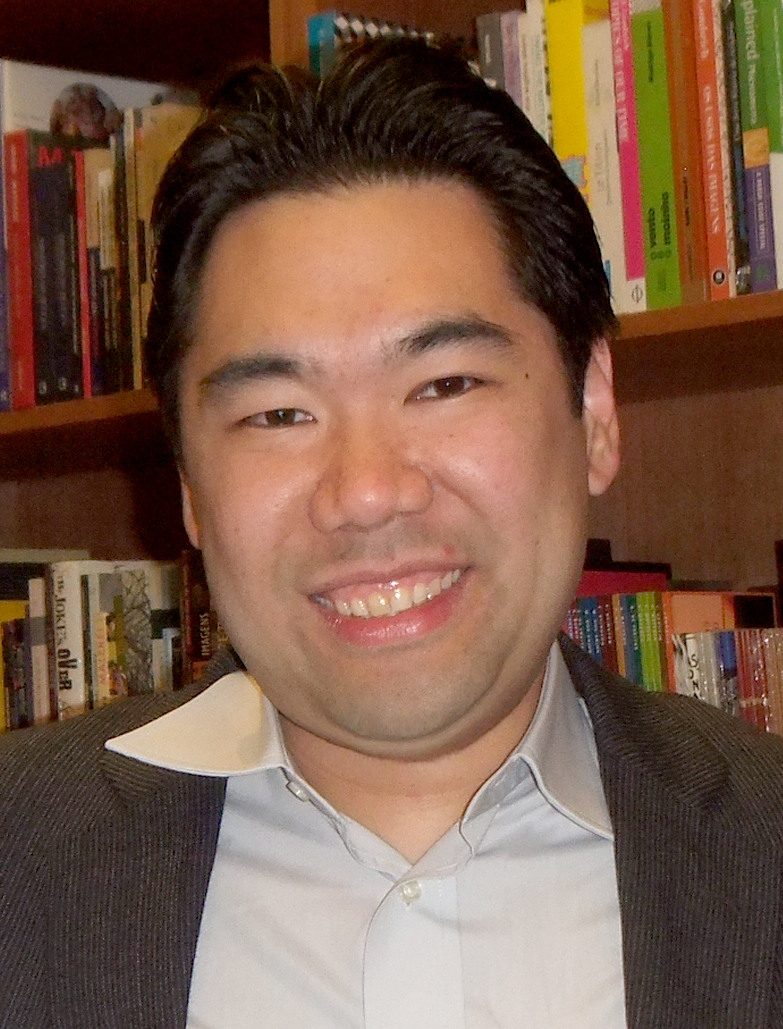
\includegraphics[width=40mm]{images/foto_leandro.jpg}
\parbox[b]{0.6\textwidth}{\textbf{Leandro Key Higuchi Yanaze}\\ \\
Contact: leyanaze@gmail.com
}

Undergraduated in architecture and urbanism, specialist in Theory and Practice of Communication, master in Social Communication and doctoral student in Electronic Systems at the Polytechnic School of University of São Paulo. Is a researcher at POLI-EDU, a research group that promotes reflection on teaching and learning  in/to engineering. He is a professor in the Methodist University of São Paulo. It is also a business consultant in the development of evaluation and measurement of communication and marketing systems.
\\ 
\noindent 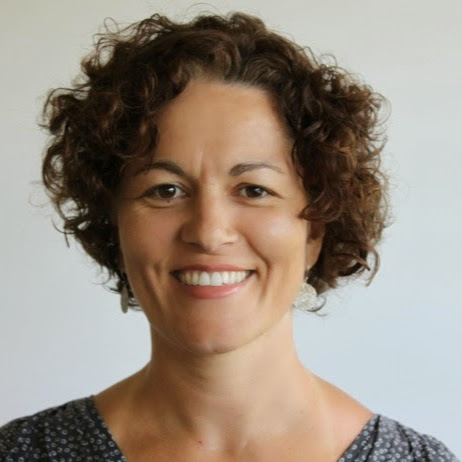
\includegraphics[width=40mm]{images/maria_alice.jpg}
\parbox[b]{0.6\textwidth}{\textbf{Maria Alice Gonzales}\\ \\
Contact: camargo.alice@gmail.com
}

Maria Alice Gonzales, researcher from The Center of Interdisciplinary of Interactive Technology and Poli-Edu, is ungraduated in architecture and urbanism. She’s doing her master degree research at The Polytechnic School of The University of São Paulo. Her research is about engineering learning spaces. She also works as a graphic and set designer.
\\

\section{Coaches}

\noindent 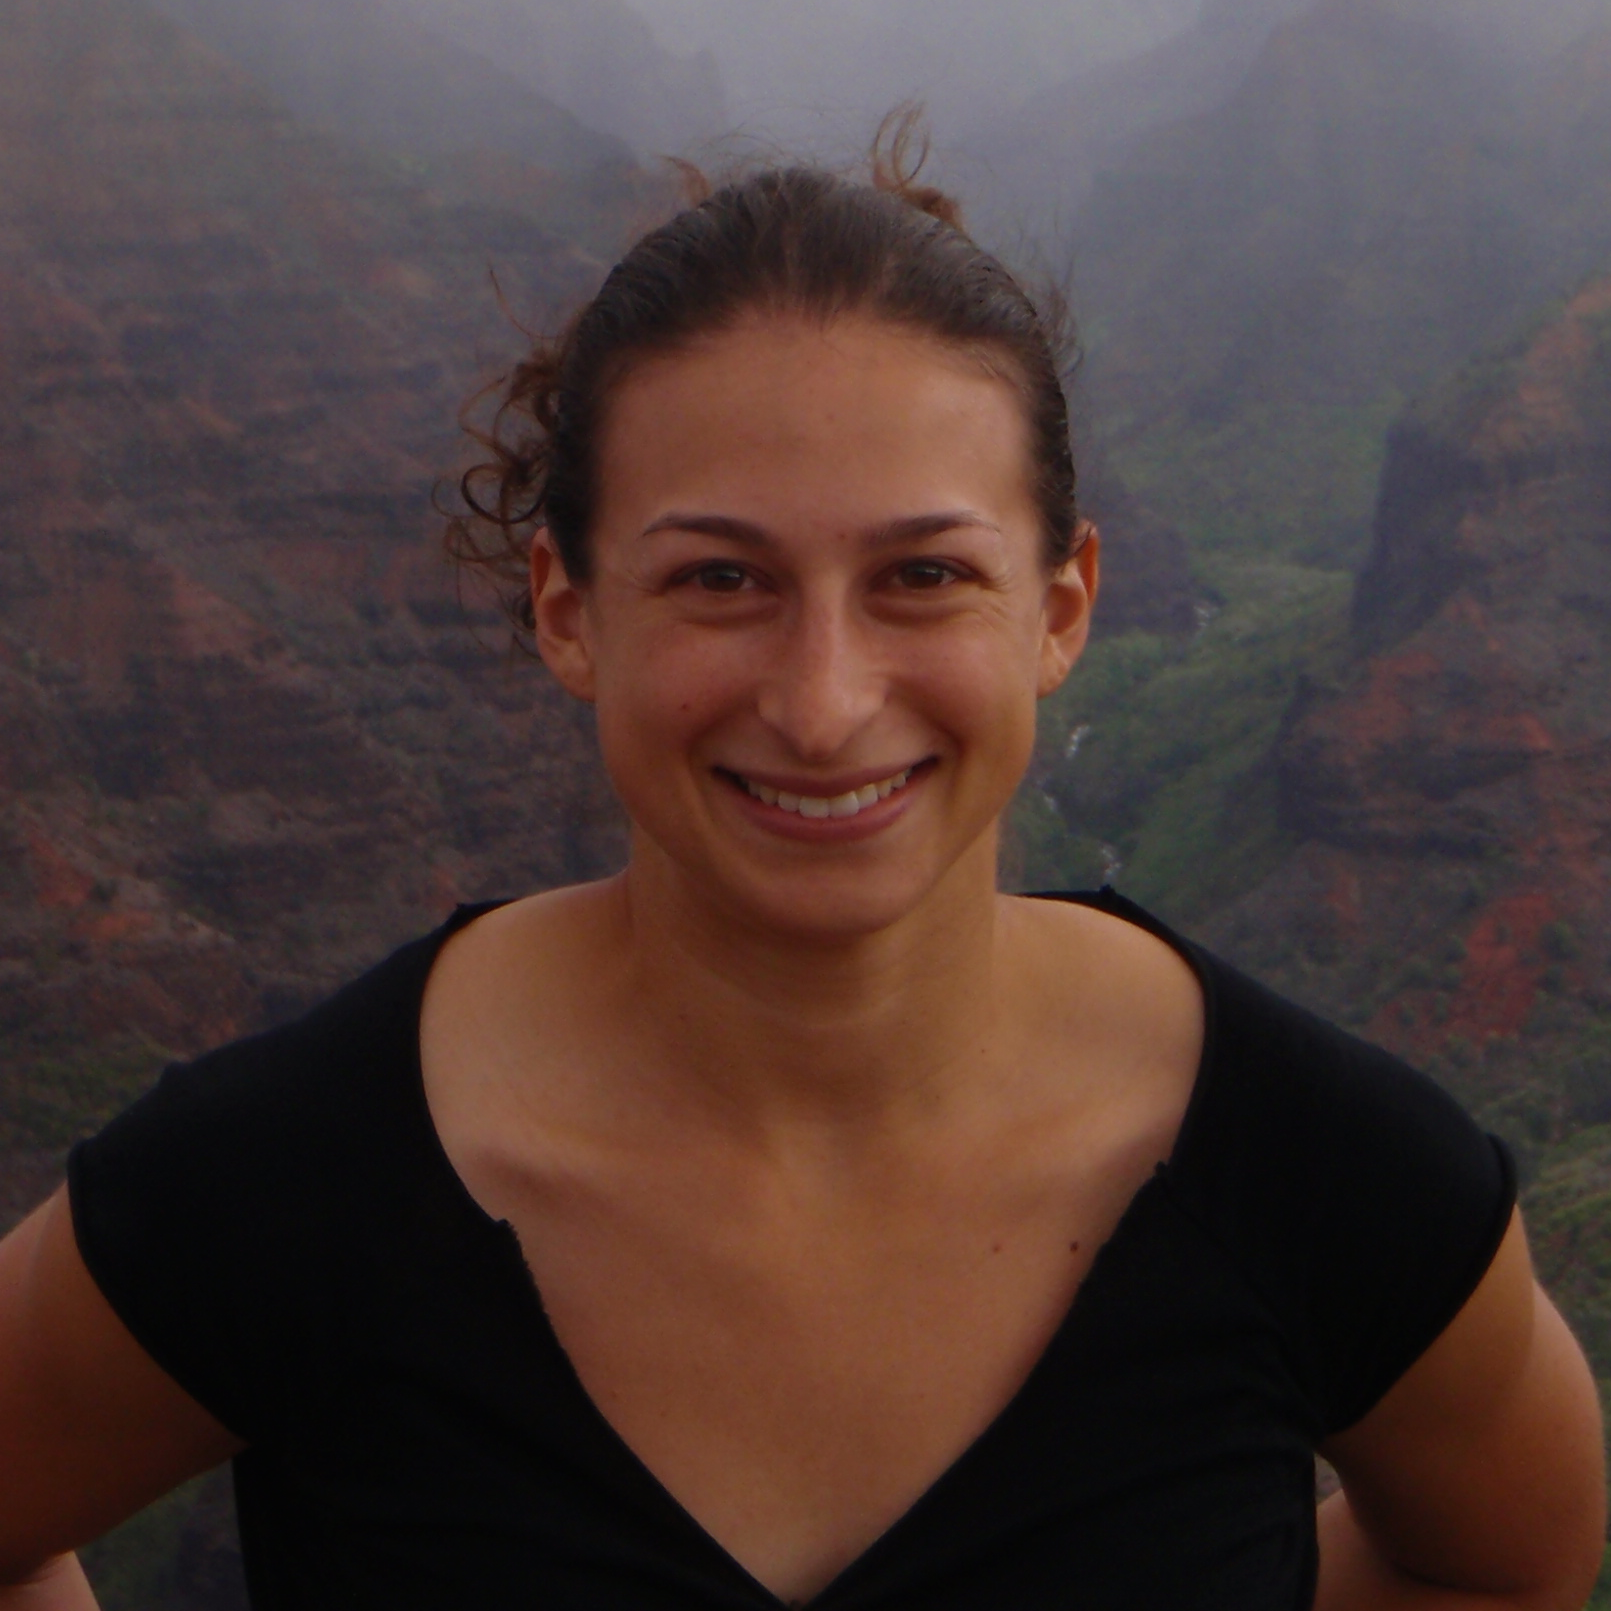
\includegraphics[width=40mm]{images/shelly.png}
\parbox[b]{0.6\textwidth}{\textbf{Shelly Goldberg}\\ \\
Contact: shelly.goldberg@gmail.com  \\
}

Shelly Goldberg was an ME310 alum from 2005, where her team worked on the EADS AugmenTable.  Shelly has been at Apple, Inc. for the past 9 years since leaving Stanford.  She is now a Senior Manager in the Mac Product Design group, where she leads a team of mechanical and product design engineers responsible for conceiving, designing, engineering, producing, and sustaining the Mac portables and desktops.  
\\

\noindent 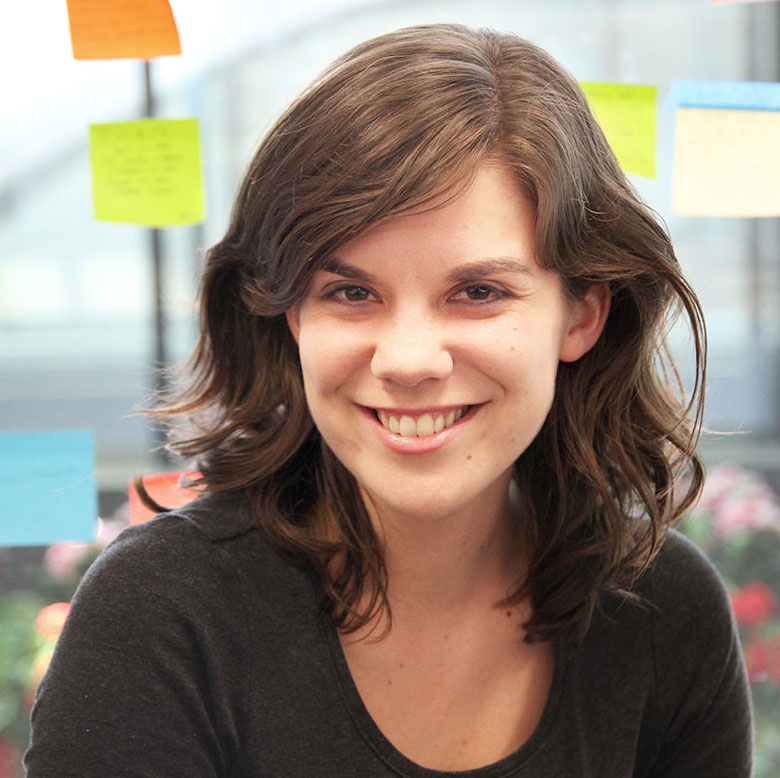
\includegraphics[width=40mm]{images/annika.jpg}
\parbox[b]{0.6\textwidth}{\textbf{Annika Matta}\\ \\
Contact: annikamatta@gmail.com  \\
}

Annika Matta is a former ME310 student and course assistant with a background in product and user experience design. As an ME310er she worked with SAP to build the Nib, a tablet with a writing experience reminiscent of paper. She graduated in 2013 and now works as a user interface designer at a consumer software startup in the Bay Area.
\\ 

